\documentclass[11pt]{article}

% First load extension packages
\usepackage[a4paper,margin=25mm]{geometry}    % page layout
\usepackage{setspace} \onehalfspacing         % line spacing
\usepackage{amsfonts,amssymb,amsmath}         % useful maths extensions
\usepackage{graphicx}                         % graphics import
\usepackage{siunitx}                          % easy SI units
\usepackage{cite}                             % better citations
\usepackage{hyperref}                         % hyperlinking
\usepackage{float}
\usepackage{adjustbox}
\usepackage{booktabs}
\usepackage{tabularx}
\usepackage{makecell}
\usepackage{tikz}
\usetikzlibrary{shapes.geometric, arrows.meta, positioning}
\newcolumntype{Y}{>{\raggedright\arraybackslash}X}
\newcolumntype{Z}{>{\raggedright\arraybackslash}X}

% Change paragraph indentation
\setlength{\parskip}{8pt}
\setlength{\parindent}{0pt}

% User-defined commands
\newcommand{\diff}[2]{\frac{\mathrm{d}{#1}}{\mathrm{d}{#2}}}
\newcommand{\ddiff}[2]{\frac{\mathrm{d}^2{#1}}{\mathrm{d}{#2}^2}}
\newcommand{\pdiff}[2]{\frac{\partial{#1}}{\partial{#2}}}
\newcommand{\pddiff}[2]{\frac{\partial^2{#1}}{\partial{#2}^2}}
\newcommand{\pdiffdiff}[3]{\frac{\partial^2{#1}}{\partial{#2}\partial{#3}}}
\renewcommand{\vec}[1]{\boldsymbol{#1}}
\newcommand{\Idx}{\;\mathrm{d}x}
\newcommand{\Real}{\mathbb{R}}
\newcommand{\Complex}{\mathbb{C}}
\newcommand{\Rational}{\mathbb{Q}}
\newcommand{\Integer}{\mathbb{Z}}
\newcommand{\Natural}{\mathbb{N}}

% topmatter
\title{Cognitive AI Coursework:  Integrating brain-inspired constraints in neural network models.}
\author{Dan Padian}
\date{\today}

% main body
\begin{document}
\maketitle

\tableofcontents
\newpage

%=============================================================================
% QUESTION 1: CRITICAL DISCUSSION (Max 4 pages total for a, b, c, d)
%=============================================================================
\section{Question 1: Brain-Inspired Constraints in Neural Networks}
\label{sec:question1}

% Critically discuss how changes to architecture, cost function, learning rule,
% and other factors can impose brain-like constraints on ANNs.
% Use equations and figures where helpful.
% Max 4 pages TOTAL for all subsections combined.

%-----------------------------------------------------------------------------
\subsection{Architecture [5 marks]}
\label{sec:q1_architecture}

Architectural modifications impose biologically grounded constraints by altering the structure and dynamics of artificial neural networks (ANNs). Whereas standard ANNs prioritise flexibility and ease of optimisation, biologically inspired architectures trade some of this flexibility to capture key organisational principles of real neural circuits.

Standard RNNs update their hidden state in discrete steps, which does not fully reflect the continuous, leaky integration of biological neurons. Leaky RNNs address this by introducing a membrane time constant $\tau$ that governs the rate at which activity decays relative to how much new input is incorporated:
\begin{equation}
a(t) = a(t-1) + \frac{\Delta t}{\tau}\Big[-a(t-1) + f\big(W_{x \to a} x(t) + W_{a \to a} a(t-1) + b_1\big)\Big].
\end{equation}
The parameter $\tau$ therefore sets the effective temporal scale of each unit: smaller values produce fast, input-driven dynamics, whereas larger values enable slow, sustained integration. This mirrors functional differences observed in the brain, where sensory areas respond rapidly to changing inputs while higher-order regions integrate information over longer timescales for working memory and decision-making.

A second biological principle is Dale’s law, which states that a neuron is either exclusively excitatory or exclusively inhibitory across all its outputs \cite{Song2016}. This can be implemented by enforcing fixed weight signs after each update:
\begin{equation}
W^{\text{rec}} = W^{\text{rec},+} \odot D,
\end{equation}
where $W^{\text{rec},+}$ is the rectified recurrent weight matrix and $D$ is a diagonal matrix with $D_{ii}=+1$ for excitatory units and $D_{ii}=-1$ for inhibitory units. Typical cortical ratios (e.g., 80\% excitatory, 20\% inhibitory) may be used or adjusted depending on the targeted brain region. Enforcing Dale’s law promotes excitatory--inhibitory balance and prevents units from arbitrarily switching signs, thereby encouraging stable recurrent computation through coordinated population dynamics.

Finally, biological neural circuits exhibit sparse connectivity: cortical neurons synapse onto only a small fraction of their potential targets (often $\sim20\%$). This can be modelled using binary masks:
\begin{equation}
W^{\text{rec}}_{\text{sparse}} = W^{\text{rec}}_{\text{dense}} \odot M,
\end{equation}
where $M_{ij} \in \{0,1\}$ specifies which connections are permitted. Sparse connectivity reduces the number of free parameters, improves interpretability by making information pathways explicit, and forces the network to develop structured representations under realistic wiring constraints.

In summary, these architectural modifications capture three core features of biological computation: temporal integration through membrane time constants, stable dynamics via excitatory--inhibitory balance, and structured information flow enabled by sparse anatomical connectivity.


% Discuss architectural constraints that make networks more brain-like:
% - Leaky integration / time constants
% - Dale's principle (E/I separation)
% - Sparse connectivity
% - Recurrent vs feedforward
% - Cell types and structured connectivity

% Examples:
% - Leaky RNN dynamics
% - E/I neuron separation
% - Sparse masks

% References: Song et al., 2016; Liu & Wang, 2024; course notes Week 4B

%-----------------------------------------------------------------------------
\subsection{Cost Function [5 marks]}
\label{sec:q1_cost}

The cost function is where biological constraints can be imposed most directly, as it dictates which network configurations are preferred during optimisation. By adding appropriate regularisation terms, learning can be steered towards operating regimes that more closely resemble those of biological neural circuits.

As noted in Section~\ref{sec:q1_architecture}, biological networks exhibit sparse connectivity and relatively low firing rates (often $<20$ Hz) due to metabolic constraints. These properties can be encouraged in artificial networks through regularisation penalties. First, L1 regularisation on synaptic weights promotes sparse connectivity \cite{yang2019}:
\begin{equation}
J = J_{\text{task}} + \beta_{\text{L1,weight}} \sum_{i,j} |w_{i \to j}|.
\end{equation}
The absolute-value penalty pushes many weights toward zero, yielding connectivity matrices in which only essential links remain. Unlike fixed architectural masks (Section~\ref{sec:q1_architecture}), this approach allows the network to \emph{learn} which connections to prune, with $\beta_{\text{L1,weight}}$ controlling the sparsity--performance trade-off.

Second, L2 regularisation on firing rates captures the metabolic cost of neural activity:
\begin{equation}
J = J_{\text{task}} + \beta_{\text{L2,rates}} \sum_{t=1}^{T} \sum_{i=1}^{N} a_{i,t}^2.
\end{equation}
Because activity is penalised quadratically, the network is encouraged to maintain low-amplitude firing while still supporting task-relevant dynamics. This tends to smooth hidden-state trajectories, prevent runaway excitation, and promotes stable recurrent computation.

Biological connectivity is also shaped by spatial structure: empirical studies show that connection probability decays exponentially with physical distance \cite{achterberg2023}. This can be modelled by embedding units in Euclidean space and penalising long-range connections:
\begin{equation}
J = J_{\text{task}} + \beta_{\text{WD}} \sum_{i,j} |w_{i \to j}| \times d_{i \to j},
\end{equation}
where $d_{i \to j}$ is the inter-unit distance. This encourages predominantly local wiring while permitting sparse long-range projections when functionally necessary, mirroring cortical organisation in which short-range connectivity dominates but strategic long-range links support inter-area communication.

Each regularisation term introduces trade-offs: excessively strong L1 penalties can prune connections essential for task performance, whereas weak penalties impose little biological structure; large L2 penalties may suppress necessary transient responses and exacerbate vanishing gradients; and distance-based penalties depend sensitively on the chosen spatial embedding and decay profile. In practice, the $\beta$ hyperparameters must be tuned to balance biological realism against accuracy. Taken together, these cost-function terms provide complementary mechanisms for steering networks toward biologically plausible regimes—enforcing sparse wiring, low metabolic activity, and realistic spatial structure—while remaining fully compatible with gradient-based optimisation.


\subsection{Learning Rule [5 marks]}
\label{sec:q1_learning}

The learning rule determines how synaptic weights change in response to activity and error signals, making it central to biological plausibility. Standard backpropagation through time (BPTT) is powerful but biologically unrealistic because it requires perfectly symmetric forward and backward weights (the weight transport problem). In the brain, no mechanism exists for copying synaptic strengths so precisely. Feedback alignment \cite{lillicrap2016} addresses this by replacing $W^{\top}$ with a fixed, randomly initialised feedback matrix $B$:
\begin{equation}
\Delta W \propto B \delta \quad \text{instead of} \quad W^{\top} \delta.
\end{equation}
During training, the forward weights gradually align with the random feedback pathways, allowing $B\delta$ to approximate true gradients and removing the need for biologically implausible symmetric connectivity.

A more physiologically grounded alternative is the dendritic error model \cite{sacramento2018}, motivated by the distinct somatic and dendritic compartments of pyramidal neurons. Here, dendrites encode error signals while the soma handles forward integration, enabling both to coexist within the same neuron:
\begin{equation}
\frac{dW_1}{dt} = \alpha \left( g(x_2) - g(\delta_2) \right) x_1,
\end{equation}
where $g$ is a nonlinearity, $x_2$ is dendritic input, $\delta_2$ is the error signal, and $x_1$ is presynaptic activity. This formulation avoids the weight transport problem and the non-locality of standard backprop, and it requires no separate inference and learning phases—both arise naturally from the same circuit dynamics.

Each approach has limitations. Feedback alignment’s fixed random feedback may struggle with deep networks or fine-grained credit assignment, and alignment emerges only gradually. Dendritic error models rely on specific cellular architecture and may not generalise across all network designs. Nonetheless, both significantly increase biological plausibility while retaining effective task learning.

% Discuss biologically plausible learning rules:
% - Weight transport problem in backprop
% - Feedback alignment
% - RFLO (Random Feedback Local Online)
% - Hebbian learning
% - STDP (Spike-Timing-Dependent Plasticity)
% - Three-factor learning rules

% Key issue: Backprop uses W^T which is biologically unrealistic
% Solutions: Random feedback weights, local learning

% References: Lillicrap et al., 2016; Murray, 2019; Whittington & Bogacz, 2019

%-----------------------------------------------------------------------------
\subsection{Other Constraints [5 marks]}
\label{sec:q1_other}

Beyond architectural, cost-function, and synaptic-level mechanisms, the learning paradigm itself imposes additional biological constraints. Three approaches—curriculum learning, three-factor learning rules, and reinforcement learning—capture principles of developmental progression, neuromodulatory control, and reward-driven adaptation that supervised backpropagation alone cannot model.


Biological learners acquire abilities gradually, mastering simpler behaviours before more complex ones. Curriculum learning formalises this by presenting training examples in an ordered progression—from short, high signal-to-noise sequences to longer or noisier inputs as training stabilises. This staged exposure encourages robust representations, reduces early overfitting, and mirrors developmental trajectories in which sensory systems mature before higher-order cortical areas.

Hebbian plasticity alone is indiscriminate: correlated activity always drives synaptic change. In the brain, plasticity is gated by neuromodulators such as dopamine and acetylcholine, which determine whether correlation leads to lasting modifications \cite{fremaux2016neuromodulated,kusmierz2017learning}. This can be expressed as
\begin{equation}
\dot{w}_{ij} = y \cdot H(\text{pre}_i, \text{post}_j),
\end{equation}
where $y$ is a neuromodulatory signal and $H$ a Hebbian term. Only when $y>0$ does learning occur. Neuromodulatory gradients across cortex \cite{froudist2023gradients} explain why some regions remain highly plastic. In ANNs, this principle is implemented by modulating weight updates with a scalar gating signal linked to reward, salience, or novelty, preventing indiscriminate learning while preserving gradient-based optimisation.


Supervised learning assumes explicit targets—a biologically implausible teaching signal. Reinforcement learning replaces these with scalar rewards, directly paralleling dopaminergic reward prediction error (RPE) signals \cite{schultz1997neural,sutton2018reinforcement}. In temporal-difference learning,
\begin{equation}
V(s_t) \leftarrow V(s_t) + \alpha \big[r_{t+1} + \gamma V(s_{t+1}) - V(s_t)\big],
\end{equation}
the bracketed term corresponds to the RPE encoded by midbrain dopamine neurons. Q-learning extends this to action values:
\begin{equation}
Q(s_t,a_t) \leftarrow Q(s_t,a_t) + \alpha \big[r_{t+1} + \gamma \max_{a'} Q(s_{t+1},a') - Q(s_t,a_t)\big].
\end{equation}
Deep RL methods such as DQN incorporate biologically inspired mechanisms including \emph{experience replay}, akin to hippocampal replay during sleep \cite{wilson1994reactivation}, and stochastic exploration policies reflecting behavioural variability. Model-based RL further aligns with hippocampal–prefrontal interactions supporting planning \cite{wang2018prefrontal}.


Together, these learning-paradigm constraints shape \emph{when}, \emph{how}, and \emph{from what signals} networks learn. Curriculum learning structures difficulty to support gradual skill acquisition; three-factor rules gate plasticity based on behavioural relevance; and reinforcement learning replaces omniscient supervision with sparse rewards that mirror dopaminergic teaching signals. These mechanisms complement earlier architectural and cost-function constraints by aligning training procedures with the temporal, modulatory, and reward-driven nature of biological learning.



%=============================================================================
% QUESTION 2: PRACTICAL IMPLEMENTATION
%=============================================================================
\newpage
\section{Question 2: NeuroGym Task Implementation}
\label{sec:question2}


\subsection{Question 2a: Model Implementation [10 marks / 3 pages]}
\label{sec:question2a}

% Initially, train and compare at least two models:
% 1. Standard RNN (vanilla, leaky, GRU, LSTM)
% 2. Brain-inspired variant(s) based on Q1 discussion

\subsubsection{Task Selection: ReadySetGo}

The ReadySetGo task \cite{remington2018flexible} requires models to measure and reproduce temporal intervals, testing temporal processing capabilities crucial for cognitive function. 

\textbf{Task Structure:} $\text{Ready}(t_0) \to \text{Set}(t_0 + t_s)
  \to \text{Go}(t_0 + t_s + g \cdot t_s)$



\begin{figure}[h]
    \centering
    \includegraphics[width=0.75\textwidth]{figures/readysetgo_task_structure.png}
    \caption{ReadySetGo task structure. Left: Input stimuli showing Ready and Set cues for three trials with different sample intervals.}
    \label{fig:task_structure}
\end{figure}

The model must measure the Ready-to-Set interval ($t_s$) and reproduce it scaled by gain factor $g = 1.5$. This requires temporal integration over variable delays (500-2000ms), directly testing the time constants and firing rate regularisation discussed in Question 1. The task was chosen because it mirrors interval timing in prefrontal cortex \cite{remington2018flexible}, isolates temporal processing from confounding working memory demands, and is sensitive to biological constraints whilst remaining computationally tractable. 


\subsubsection{Model Architectures}


\textbf{Model 1: Vanilla RNN (Baseline)}

Standard recurrent architecture with tanh activation function. The tanh activation was chosen for its bounded output range $[-1, 1]$, which prevents explosive activations whilst allowing both positive and negative values. This serves as the baseline against which biological constraints are evaluated.

\textbf{Model 2: Leaky RNN}

Incorporates membrane time constant $\tau = 100$ms for temporal integration, directly implementing the architectural constraint discussed in Section \ref{sec:q1_architecture}. The leaky integration term allows the network to maintain information across delays by controlling the timescale of hidden state decay. This is particularly relevant for ReadySetGo, where accurate interval timing requires sustained temporal representations. Recurrent noise ($\sigma_{\text{rec}} = 0.15$, $\xi_t \sim \mathcal{N}(0,1)$) is added to match neural variability observed in biological systems. The activation function is changed to ReLU to maintain non-negative firing rates, consistent with biological neurons.

\textbf{Model 3: Leaky RNN + Feedback Alignment}

Builds on Model 2 by addressing the weight transport problem through feedback alignment \cite{lillicrap2016}, as discussed in Section \ref{sec:q1_learning}. Forward propagation uses trained weights $W$, whilst backpropagation uses fixed random weights $B$ instead of the biologically implausible symmetric transpose $W^T$. This removes the requirement for reciprocal connectivity whilst maintaining effective gradient-based learning.

\textbf{Model 4: Biologically Realistic RNN}

Integrates all Question 1 constraints for maximal biological realism: (1) feedback alignment with random backward weights addressing the weight transport problem, (2) Dale's principle enforcing 80\% excitatory / 20\% inhibitory separation matching cortical ratios, (3) L1 weight regularisation ($\beta_{L1} = 10^{-5}$) promoting learned sparse connectivity, and (4) L2 firing rate regularisation ($\beta_{L2} = 0.01$) enforcing metabolically plausible activity levels. This architecture combines constraints across learning (feedback alignment), structure (Dale's principle, time constants), and optimization (L1/L2 regularisation) to test whether biological plausibility impairs task performance.

\begin{figure}[H]
\centering
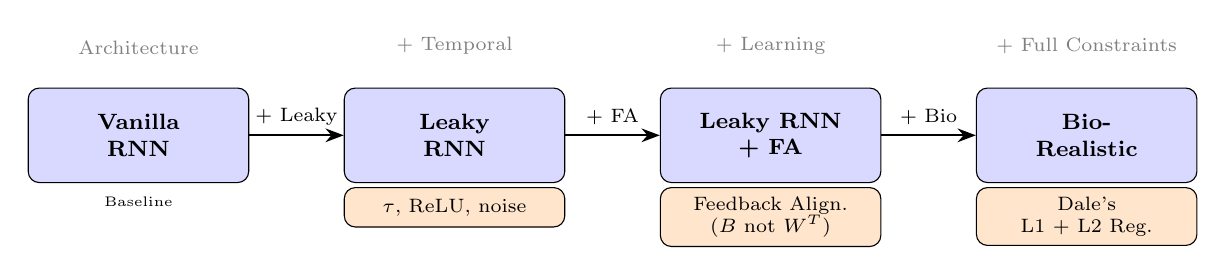
\begin{tikzpicture}[
    model/.style={rectangle, rounded corners, minimum width=2.8cm, minimum height=1.2cm,
                  text centered, draw=black, fill=blue!15, font=\bfseries\footnotesize, align=center},
    constraint/.style={rectangle, rounded corners, minimum width=2.8cm, minimum height=0.5cm,
                       text centered, draw=black, fill=orange!20, font=\scriptsize, align=center},
    arrow/.style={-Stealth, thick, black},
    label/.style={font=\tiny, align=center},
    node distance=0.3cm
]

% Model 1
\node (m1) [model] {Vanilla\\RNN};
\node (c1) [below=0.05cm of m1, label] {Baseline};

% Arrow 1
\node (arrow1) [right=1.2cm of m1] {};
\draw [arrow] (m1) -- node[above, font=\scriptsize] {+ Leaky} (arrow1);

% Model 2 with constraints below
\node (m2) [model, right=1.2cm of m1] {Leaky\\RNN};
\node (m2c) [constraint, below=0.05cm of m2] {$\tau$, ReLU, noise};

% Arrow 2
\node (arrow2) [right=1.2cm of m2] {};
\draw [arrow] (m2) -- node[above, font=\scriptsize] {+ FA} (arrow2);

% Model 3 with constraints below
\node (m3) [model, right=1.2cm of m2] {Leaky RNN\\+ FA};
\node (m3c) [constraint, below=0.05cm of m3] {Feedback Align.\\($B$ not $W^T$)};

% Arrow 3
\node (arrow3) [right=1.2cm of m3] {};
\draw [arrow] (m3) -- node[above, font=\scriptsize] {+ Bio} (arrow3);

% Model 4 with constraints below
\node (m4) [model, right=1.2cm of m3] {Bio-\\Realistic};
\node (m4c) [constraint, below=0.05cm of m4] {Dale's\\L1 + L2 Reg.};

% Top labels
\node[above=0.3cm of m1, font=\scriptsize, text=gray] {Architecture};
\node[above=0.3cm of m2, font=\scriptsize, text=gray] {+ Temporal};
\node[above=0.3cm of m3, font=\scriptsize, text=gray] {+ Learning};
\node[above=0.3cm of m4, font=\scriptsize, text=gray] {+ Full Constraints};

\end{tikzpicture}
\caption{Progressive addition of biological constraints across four model architectures. Each model builds on the previous by adding brain-inspired mechanisms: temporal integration (Model 2), biologically plausible learning (Model 3), and full architectural constraints (Model 4).}
\label{fig:model_progression}
\end{figure}


\subsubsection{Implementation Details}

All models were trained for 2,000 steps using identical hyperparameters to ensure fair comparison: Adam optimizer ($\alpha = 0.001$), 50 hidden units, batch size 16, temporal discretization $\Delta t = 20$ms, and recurrent noise $\sigma_{\text{rec}} = 0.15$. Class weights $(0.1, 1.0)$ were applied to balance the fixation/action imbalance inherent in timing tasks. The loss function combined cross-entropy task loss with L1 weight regularisation ($\beta_{L1} = 10^{-4}$) and L2 activity regularisation ($\beta_{L2} = 0.01$) for the bio-realistic model only.

\textbf{Feedback Alignment Implementation.}
Implementing biologically plausible feedback alignment in PyTorch required careful consideration of the autograd system. Standard PyTorch hooks proved insufficient because they cannot override gradient computation during the backward pass in a way that properly implements random feedback weights. The solution involved creating a custom \texttt{torch.autograd.Function} that explicitly separates forward and backward passes:

\textbf{Forward pass:} Standard linear transformation using trained weights $W$:
\begin{equation}
y = xW^{\top} + b
\end{equation}

\textbf{Backward pass:} Replace $W^{\top}$ with fixed random matrix $B$ for input gradients whilst maintaining standard gradients for weight updates:
\begin{equation}
\frac{\partial L}{\partial x} = \frac{\partial L}{\partial y} \cdot B, \quad \frac{\partial L}{\partial W} = \left(\frac{\partial L}{\partial y}\right)^{\top} x
\end{equation}

This ensures forward weights learn through standard backpropagation whilst error signals propagate through random feedback pathways—solving the weight transport problem. The feedback matrix $B \in \mathbb{R}^{d_{\text{in}} \times d_{\text{out}}}$ was initialized uniformly: $B_{ij} \sim \mathcal{U}\left(-\frac{1}{\sqrt{d_{\text{in}}}}, \frac{1}{\sqrt{d_{\text{in}}}}\right)$, matching the scale of forward weights to prevent gradient explosion. Initial implementations using hooks on input tensors failed because PyTorch's autograd graph construction does not allow runtime modification of gradient flow in recurrent settings. The custom Function approach succeeded by explicitly overriding \texttt{backward()}, giving full control over gradient routing whilst maintaining compatibility with Adam optimisation and gradient clipping.

\subsubsection{Learning Performance}

\begin{figure}[H]
    \centering
    \includegraphics[width=0.75\textwidth]{figures/question_2a_results.png}
    \caption{Learning curves showing task loss only for fair comparison across models. All models successfully learn the timing task, demonstrating that biological constraints (feedback alignment, Dale's principle, L1/L2 regularisation) do not impair task performance. The bio-realistic model achieves comparable task loss despite additional constraints.}
    \label{fig:learning_curves}
\end{figure}

All models converge successfully, with every architecture achieving low task loss ($<0.04$), demonstrating that biological constraints are compatible with effective learning on temporal tasks. The Vanilla RNN (blue) converges fastest initially, benefiting from unconstrained optimization, though after 1,500 steps the Leaky and Bio-realistic models match or exceed its performance. Feedback alignment impairs early learning, as the Leaky+FA model (green) shows consistently higher loss than the standard Leaky RNN (orange) throughout training, indicating that random backward weights slow convergence compared to symmetric backpropagation—though both reach similar final performance. Despite integrating four constraints (FA, Dale's, L1, L2), the Bio-realistic model (red) converges to comparable task loss as simpler architectures and notably outperforms Leaky+FA, suggesting that Dale's principle and regularisation improve learning dynamics rather than hindering them. Finally, plotting task loss rather than total loss is essential for fair comparison, as the Bio-realistic model's total loss includes L1 weight and L2 activity penalties that would artificially inflate apparent performance gaps despite equivalent task competence.  

%-----------------------------------------------------------------------------  
% QUESTION 2B: ANALYSIS OF TRAINED MODELS (Max 4 pages)
%-----------------------------------------------------------------------------
\newpage
\subsection{Question 2b: Hidden Unit Activity Analysis [20 marks / 4 pages]}
\label{sec:question2b}

% Analyze how trained models solve the task
% Compare models and interpret differences

\subsubsection{Performance Comparison}

Figure \ref{fig:timing_performance} exposes distinct timing strategies beyond simple loss metrics. The Vanilla RNN (blue) shows consistent linear scaling but systematically undershoots targets, learning relative timing structure without precise calibration. The Leaky RNN (orange) achieves near-perfect performance ($\mu=-19.4$ms, $\sigma=195.5$ms), with leaky dynamics ($\tau=100$ms) providing an intrinsic timescale for accurate interval representation. In stark contrast, Leaky+FA (green) exhibits severe underprediction ($\mu=-324.6$ms, $\sigma=173.2$ms)—feedback alignment's random backward weights impair precise temporal mapping, so the model learns \textit{when} to respond but not \textit{exactly when}.

Most intriguingly, the Bio-Realistic model (red) displays bimodal behaviour: complete response failures (zero cluster) and delayed successful responses ($\mu=203.6$ms, $\sigma=873.7$ms). This pattern mirrors biological neural variability in primate timing tasks \cite{remington2018}, where L1 regularisation causes failures when critical neurons remain silent, whilst Dale's principle introduces noise manifesting as reaction delays. Accuracy metrics alone would miss these nuanced differences, highlighting the importance of direct interval analysis.

\begin{figure}[H]
    \centering
    \includegraphics[width=0.9\textwidth]{figures/readysetgo_timing.png}
    \caption{Timing performance analysis across models. \textbf{Left:} Scatter plot showing target versus produced intervals, with black diagonal indicating perfect timing. Leaky RNN (orange) clusters near-perfectly along the diagonal, whilst Leaky+FA (green) systematically undershoots and Bio-Realistic (red) shows high variance with failure modes. \textbf{Right:} Error distributions with mean ($\mu$) and standard deviation ($\sigma$) revealing systematic biases and precision differences. Fixed 50ms bin width enables direct comparison across models.}
\label{fig:timing_performance}
\end{figure}

\subsubsection{Neural Population Dynamics}

Figure \ref{fig:trajectories} reveals fundamentally different computational strategies by visualising how 50-dimensional neural activity evolves through PCA space during timing. The Vanilla RNN exhibits a single, deterministic trajectory (PC1: 70.4\%, PC2: 24.6\%), suggesting simple attractor dynamics where neural state flows along a fixed manifold. This low-dimensional simplicity explains systematic timing errors—the singular path cannot flexibly represent multiple interval durations.

The Leaky RNN shows 10-15 distinct, smooth parallel trajectories (PC1: 62.1\%, PC2: 20.3\%), resembling primate prefrontal cortex dynamics \cite{remington2018} where different intervals occupy separate paths through a shared neural manifold. Leaky integration ($\tau=100$ms) enables richer temporal representations whilst maintaining structured, low-noise dynamics. Leaky+FA displays similar structure but with higher compression (PC1: 84.2\%, PC2: 13.0\%)—feedback alignment's random backward weights regularise dynamics to lower dimensionality, potentially explaining systematic timing bias through reduced interval discrimination.

Most strikingly, the Bio-Realistic model exhibits irregular, variable trajectories with no parallel structure (PC1: 86.6\%, PC2: 8.3\%). Dale's principle and L1 regularisation create sparse, intermittent activity producing jagged paths that mirror biological circuit recordings \cite{remington2018}. Counterintuitively, high PC1 variance reflects \textit{sparsity}, not low dimensionality.

Critically, across models, Ready and Go occupy consistent state space regions whilst Set positions vary dramatically, suggesting interval duration is encoded geometrically: spatial position along a neural manifold directly represents elapsed time—a population clock mechanism \cite{remington2018}.

\begin{figure}[H]
    \centering
    \includegraphics[width=0.9\textwidth]{figures/readysetgo_trajectories.png}
    \caption{Neural trajectories in PCA space (10 trials per model). Green circles mark Ready (trial start), blue diamonds mark Set (cue), red squares mark Go (response).}
    \label{fig:trajectories}
\end{figure}

\subsubsection{Temporal Activity Patterns}

Figure \ref{fig:heatmaps} reveals how individual neurons encode timing across trial duration. The Vanilla RNN exhibits binary activation patterns—neurons are either strongly active or silent—creating blocky structure before Set (red line), then transitioning to dense, sustained firing where nearly all neurons activate at staggered phases. This distributed, continuous coding uses the full population but lacks temporal precision. The Leaky RNN maintains dense activity but with shorter, more structured bursts, whilst Leaky+FA concentrates firing around Set, showing increased sparsity. Most strikingly, the Bio-Realistic model activates only ~9 neurons clustered near Set—extreme sparsity enforced by L1 regularization, where most of the 50-neuron population remains silent throughout.

This sparsity gradient is biologically significant. Cortical recordings show only 10-20\% of neurons fire in any time window \cite{remington2018}, making the Bio-Realistic model's sparse activation the most faithful representation. Dense firing in Vanilla/Leaky models is metabolically expensive and unlike biology, where energy constraints favour sparse codes. However, sparsity creates fragility: the Bio-Realistic model's reliance on ~9 critical neurons explains its response failures—if these neurons don't activate, timing collapses. This demonstrates the biological trade-off between metabolic efficiency (sparsity) and robustness (redundancy), where evolution balances sparse coding's efficiency against failure risk through partially overlapping neural populations. 

\begin{figure}[H]
    \centering
    \includegraphics[width=0.9\textwidth]{figures/readysetgo_heatmaps.png}
    \caption{Activity heatmaps showing 50 neurons over time for a single trial across models. Cyan dashed line marks Set cue, lime dashed line marks expected Go response. Vertical axis: neuron index, horizontal axis: time, color: activity magnitude. }
    \label{fig:heatmaps}
\end{figure}

\subsubsection{Neuron Importance Analysis}

\textcolor{red}{change this plot to be a histogram of percentage contributed of activations}

Figure \ref{fig:neuron_importance} quantifies functional specialization by ranking neurons by activity variance—a proxy for how much timing information each unit carries. The Bio-Realistic model (red) exhibits an extremely steep importance curve: after the top 10 neurons, contributions collapse, indicating that a small, highly specialized “timing circuit” explains nearly all variance. In contrast, the Vanilla RNN (blue) distributes computation broadly, requiring roughly 35 neurons to reach 0.25 normalized variance, with no single unit playing a dominant role. The Leaky models (orange, green) lie between these extremes, with Leaky+FA showing slightly sharper concentration, suggesting that feedback-alignment’s random gradients unintentionally promote specialization. This hierarchy mirrors biological cortex, where sparse task-encoding neurons sit within larger populations \cite{remington2018}, yet it also exposes trade-offs: extreme specialization (Bio-Realistic) is efficient but fragile, distributed coding (Vanilla) is robust but metabolically and computationally costly, and intermediate strategies (Leaky) balance precision and redundancy. Together, these patterns highlight a general principle: effective neural computation must trade off specialization for efficiency against distribution for robustness, with biological constraints nudging systems toward sparse but potentially vulnerable representations.

\begin{figure}[H]
    \centering
    \includegraphics[width=0.9\textwidth]{figures/mechanism_5_neuron_importance.png}
    \caption{Neuron importance ranked by normalized activity variance across time. Bio-Realistic (red) shows extreme concentration with top 10 neurons dominating, whilst Vanilla (blue) distributes computation broadly across ~35 neurons. Leaky models (orange, green) show intermediate specialization, balancing efficiency and robustness.}
    \label{fig:neuron_importance}
\end{figure}

\subsubsection{Summary of Findings}

Analysis of trained models reveals fundamentally different computational strategies for interval timing, shaped by architectural constraints and biological principles. The Leaky RNN achieves optimal performance through parallel trajectory organization in state space and moderate neural specialization—approximately 10-15 distinct temporal trajectories encode different intervals through structured, low-noise dynamics, whilst ~20-30 neurons contribute meaningfully to timing computation. This intermediate strategy balances precision (achieving $\mu=-19.4$ms timing error) against robustness, mirroring efficient biological circuits where redundancy protects against noise whilst avoiding metabolic waste.

Biological constraints push solutions toward sparse, specialized representations at the cost of performance. The Bio-Realistic model's extreme sparsity (~9 active neurons, top 10 explaining nearly all variance) and irregular state-space trajectories closely resemble primate cortical recordings \cite{remington2018}, but this biological fidelity introduces fragility: response failures occur when critical sparse neurons remain silent, and high variance ($\sigma=873.7$ms) reflects stochastic recruitment. Conversely, the Vanilla RNN's dense, distributed coding (requiring ~35 neurons for equivalent representation) achieves robustness but sacrifices efficiency and biological plausibility. Feedback alignment further reveals that learning algorithm constraints matter: random backward weights compress dynamics to lower dimensionality, producing systematic timing bias despite accurate task structure learning.

Critically, all models encode time geometrically—Set cue position varies along neural manifolds whilst Ready and Go occupy consistent regions, implementing "population clock" mechanisms where spatial location in state space directly represents elapsed time \cite{remington2018}. This geometric temporal encoding appears to be a convergent solution across architectures, suggesting it may be a fundamental computational principle for interval timing in both artificial and biological neural systems. The findings demonstrate that biological constraints (Dale's principle, sparse coding, feedback alignment) are compatible with effective learning but introduce specific trade-offs: sparsity improves metabolic efficiency at the cost of fragility, whilst biologically-plausible learning impairs precision even when preserving task accuracy.

%-----------------------------------------------------------------------------
% QUESTION 2C: SECOND TASK (Max 4 pages)
%-----------------------------------------------------------------------------

\newpage
\subsection{Question 2c: Second Task Analysis [20 marks / 4 pages]}
\label{sec:question2c}

Now we will take the models from section \ref{sec:question2a} and will train them on a different tasks from the neuro gym library, once again analysing their performance and to see if the hidden neurons act the same way to see how the models learn to complete the task separately. 

\subsubsection{Task Description}

The second task is \texttt{MultiSensoryIntegration-v0}. Figure \ref{fig:q2_multisensory_task_structure} depicts howe ach trial presents two simultaneous sensory streams (modality 1 and modality 2), each with left/right channels. Inputs are five streams: fixation (row 1), mod1-left/right (rows 2--3), mod2-left/right (rows 4--5). A trial’s difficulty is set by (i) \textbf{coh} -- the evidence strength (higher = cleaner signal, lower = noisy) and (ii) \textbf{coh\_prop} -- the fraction of evidence assigned to modality 1 vs. modality 2 (near 1 biases mod1, near 0 biases mod2). The agent should fixate during the cue, integrate both modalities, and emit a single binary decision (The top row, green=left/red=right) when fixation ends.

\begin{figure}[H]
    \centering
    \includegraphics[width=0.95\textwidth]{figures/q2_multisensory_task_structure.png}
    \caption{Task structure (three concatenated trials): fixation, modality 1 (L/R), modality 2 (L/R), and decision band (green=left, red=right).}
    \label{fig:q2_multisensory_task_structure}
\end{figure}

The network’s job is to combine modality-specific evidence (weighted by \textbf{coh\_prop}), respect fixation, and classify left vs. right. This demands evidence integration rather than timing like the ReadySetGo task required.

\subsubsection{Training and Performance}

All four architectures from Question 2a were trained in supervised mode on \texttt{MultiSensoryIntegration-v0} via the NeuroGym dataset (cross-entropy, mini-batches, scheduled LR drops). Loss decays smoothly and stabilises by \(\sim\)8k steps (log y-axis in Fig.~\ref{fig:q2_multisensory_training_curves}.

\begin{figure}[H]
    \centering
    \includegraphics[width=0.95\textwidth]{figures/q2_multisensory_training_curves.png}
    \caption{Training loss (log scale) for all architectures; y-lim fixed to 0.05–0.20.}
    \label{fig:q2_multisensory_training_curves}
\end{figure}

\begin{table}[h!]
\centering
\small
\setlength{\tabcolsep}{12pt}
\begin{tabular}{c c c c}
\hline
\textbf{Vanilla RNN} & \textbf{Leaky RNN} & \textbf{Leaky + FA} & \textbf{Bio-realistic} \\
\hline
0.926 & 0.904 & 0.898 & 0.898 \\
\hline
\end{tabular}
\end{table}



All models reach high accuracy; vanilla is best by a small margin. FA and bio constraints impose only minor drops, showing that approximate feedback and sparse E/I structure still support reliable multisensory integration.

Confusion matrices (rows = true \{Left, Right\}, cols = pred \{Left, Right\}):
\begin{center}
\begin{tabular}{c c c c}
Vanilla & Leaky & Leaky+FA & Bio-realistic \\
$\begin{bmatrix}230 & 27 \\ 10 & 233\end{bmatrix}$ &
$\begin{bmatrix}234 & 15 \\ 33 & 218\end{bmatrix}$ &
$\begin{bmatrix}218 & 20 \\ 31 & 231\end{bmatrix}$ &
$\begin{bmatrix}210 & 19 \\ 32 & 239\end{bmatrix}$ \\
\end{tabular}
\end{center}

\subsubsection{Hidden Unit Analysis}

PCA (Fig.~\ref{fig:q2_multisensory_pca}) shows each model carves out clean left/right clusters in a low-dimensional subspace, but with different variance footprints. Vanilla packs \(\sim95\%\) into PC1–2; leaky/FA spill more into PC2; the bio model compresses hardest because of sparsity. The task geometry stays intact, yet the biologically constrained variants live in a tighter, lower-dimensional manifold. 

The PCA shows that each model’s trial averaged hidden states cluster by decision (left vs. right) in a low-dimensional space. It’s not about individual neurons being exclusively assigned to a side; rather, the population activity for left trials versus right trials occupies distinct regions along the first two principal components. 

\begin{figure}[H]
    \centering
    \includegraphics[width=0.95\textwidth]{figures/q2_multisensory_pca.png}
    \caption{PCA of per-trial mean hidden states (rows = models, colored by decision).}
    \label{fig:q2_multisensory_pca}
\end{figure}


Heatmaps (Fig.~\ref{fig:q2_multisensory_heatmaps}) highlight style differences: vanilla/leaky spread activity widely, while bio is starkly sparse (only \(\sim\)10–15/64 units ever engage, with a handful dominating at decision). Leaky/FA sit quiet through the cue then burst near decision; vanilla hums along continuously; bio stays frugal end-to-end, in line with its E/I + L1/L2 constraints. The bio model’s sparse, low-rate profile echoes cortical recordings (selective, energy-efficient), but is also less robust—performance dips if a few dominant units misfire.

\begin{figure}[H]
    \centering
    \includegraphics[width=0.95\textwidth]{figures/q2_multisensory_heatmaps.png}
    \caption{Hidden-unit activity heatmaps (correct trials, averaged) for all models.}
    \label{fig:q2_multisensory_heatmaps}
\end{figure}

Choice decoding rises near the decision window for all architectures; vanilla/leaky reach higher decoding earlier, whereas FA/bio peaks lag by \(\sim\)tens of ms, consistent with slower evidence accumulation under approximate feedback/sparsity. Overall, biological constraints mainly compress dimensionality and induce sparsity without disrupting task-relevant geometry—trading a bit of speed/robustness for neural realism.


\subsubsection{Cross-Task Comparison}


Compared to ReadySetGo timing, all models transfer well to evidence integration, but architectural constraints change the strategy: sparsity and FA reduce dimensionality and delay choice-readout timing while maintaining accuracy. The bio and FA models remain slightly less confident/earlier-decoding than vanilla on both tasks, indicating a consistent trade-off between biological plausibility and speed of reliable readout, rather than a task-specific deficit.

%-----------------------------------------------------------------------------
% QUESTION 2D: ORIGINAL CONTRIBUTION (Max 4 pages)
%-----------------------------------------------------------------------------
\subsection{Other Constraints [5 marks]}
\label{sec:q1_other}

Beyond architectural, cost-function, and synaptic-level mechanisms, the learning paradigm itself imposes additional biological constraints. Three approaches—curriculum learning, three-factor learning rules, and reinforcement learning—capture principles of developmental progression, neuromodulatory control, and reward-driven adaptation that supervised backpropagation alone cannot model.

\textbf{Curriculum Learning: Structured Task Progression.}
Biological learners acquire abilities gradually, mastering simpler behaviours before more complex ones. Curriculum learning formalises this by presenting training examples in an ordered progression—from short, high signal-to-noise sequences to longer or noisier inputs as training stabilises. This staged exposure encourages robust representations, reduces early overfitting, and mirrors developmental trajectories in which sensory systems mature before higher-order cortical areas.

\textbf{Three-Factor Learning Rules: Neuromodulated Plasticity.}
Hebbian plasticity alone is indiscriminate: correlated activity always drives synaptic change. In the brain, plasticity is gated by neuromodulators such as dopamine and acetylcholine, which determine whether correlation leads to lasting modifications \cite{fremaux2016neuromodulated,kusmierz2017learning}. This can be expressed as
\begin{equation}
\dot{w}_{ij} = y \cdot H(\text{pre}_i, \text{post}_j),
\end{equation}
where $y$ is a neuromodulatory signal and $H$ a Hebbian term. Only when $y>0$ does learning occur. Neuromodulatory gradients across cortex \cite{froudist2023gradients} explain why some regions remain highly plastic. In ANNs, this principle is implemented by modulating weight updates with a scalar gating signal linked to reward, salience, or novelty, preventing indiscriminate learning while preserving gradient-based optimisation.

\textbf{Reinforcement Learning: Reward-Driven Adaptation.}
Supervised learning assumes explicit targets—a biologically implausible teaching signal. Reinforcement learning replaces these with scalar rewards, directly paralleling dopaminergic reward prediction error (RPE) signals \cite{schultz1997neural,sutton2018reinforcement}. In temporal-difference learning,
\begin{equation}
V(s_t) \leftarrow V(s_t) + \alpha \big[r_{t+1} + \gamma V(s_{t+1}) - V(s_t)\big],
\end{equation}
the bracketed term corresponds to the RPE encoded by midbrain dopamine neurons. Q-learning extends this to action values:
\begin{equation}
Q(s_t,a_t) \leftarrow Q(s_t,a_t) + \alpha \big[r_{t+1} + \gamma \max_{a'} Q(s_{t+1},a') - Q(s_t,a_t)\big].
\end{equation}
Deep RL methods such as DQN incorporate biologically inspired mechanisms including \emph{experience replay}, akin to hippocampal replay during sleep \cite{wilson1994reactivation}, and stochastic exploration policies reflecting behavioural variability. Model-based RL further aligns with hippocampal–prefrontal interactions supporting planning \cite{wang2018prefrontal}.

\textbf{Summary.}
Together, these learning-paradigm constraints shape \emph{when}, \emph{how}, and \emph{from what signals} networks learn. Curriculum learning structures difficulty to support gradual skill acquisition; three-factor rules gate plasticity based on behavioural relevance; and reinforcement learning replaces omniscient supervision with sparse rewards that mirror dopaminergic teaching signals. These mechanisms complement earlier architectural and cost-function constraints by aligning training procedures with the temporal, modulatory, and reward-driven nature of biological learning.





\newpage
\label{sec:question2d}


%=============================================================================
% QUESTION 3: CONCLUSION (Max 500 words)
%=============================================================================
\section{Question 3: Conclusion [10 marks]}
\label{sec:question3}

% Brief discussion summarizing learnings
% Reference literature
% Max 500 words



%=============================================================================
% REFERENCES
%=============================================================================

\singlespacing
\bibliographystyle{ieeetr}
\bibliography{refs}

% Key citations to include:
% Lillicrap et al., 2016 - Feedback Alignment
% Murray, 2019 - RFLO learning
% Song et al., 2016 - Dale's principle, sparse connectivity
% Goudar et al., 2023 - L2 firing rate regularization
% Remington et al., 2018 - ReadySetGo task, neural trajectories
% Churchland et al., 2012 - Population dynamics
% Yang et al., 2019 - L1 regularization
% Achterberg et al., 2023 - Distance-based connectivity
% Whittington & Bogacz, 2019 - Dendritic error model
% Liu & Wang, 2024 - Cell types

% the end
\end{document}
